%%%%%%%%%%%%%%%%%%%%%%%%%%%%%%%%%%%%%%%%%
% Journal Article
% LaTeX Template
% Version 1.4 (15/5/16)
%
% This template has been downloaded from:
% http://www.LaTeXTemplates.com
%
% Original author:
% Frits Wenneker (http://www.howtotex.com) with extensive modifications by
% Vel (vel@LaTeXTemplates.com)
%
% License:
% CC BY-NC-SA 3.0 (http://creativecommons.org/licenses/by-nc-sa/3.0/)
%
%%%%%%%%%%%%%%%%%%%%%%%%%%%%%%%%%%%%%%%%%

%----------------------------------------------------------------------------------------
%	PACKAGES AND OTHER DOCUMENT CONFIGURATIONS
%----------------------------------------------------------------------------------------

\documentclass[14pt, a4paper]{article}
\usepackage[english, russian]{babel}
\usepackage{fontspec}
% \setmainfont{Times New Roman}

\setromanfont{Times New Roman}
\setsansfont{Arial}

% \usepackage{cyrtimes}

\usepackage{extsizes}
% \usepackage[T2A]{fontenc}
%
% \usepackage[utf8]{inputenc}

\usepackage{indentfirst}

%\usepackage{times}
\linespread{1.5}
\usepackage[left=30mm,right=15mm,top=15mm,bottom=20mm]{geometry}
\usepackage[framed,numbered,autolinebreaks,useliterate]{mcode}

\usepackage{graphicx, amsmath}
\numberwithin{figure}{section}
\graphicspath{{images/}}
\usepackage{amsfonts,amssymb}
\usepackage{caption}
\captionsetup[figure]{name=Рисунок, labelsep=endash}

\numberwithin{equation}{section}

\usepackage{booktabs} % Horizontal rules in tables

\usepackage{lettrine} % The lettrine is the first enlarged letter at the beginning of the text

\usepackage{enumitem} % Customized lists
\setlist[itemize]{noitemsep} % Make itemize lists more compact

\usepackage{listings}
\lstloadlanguages{C,[ANSI]C++,Matlab}%,Clean,make,Fortran}%Загружаемые языки
\lstset{
  language=C,                % choose the language of the code
  numbers=left,                   % where to put the line-numbers
  stepnumber=1,                   % the step between two line-numbers.
  numbersep=5pt,                  % how far the line-numbers are from the code
  backgroundcolor=\color{white},  % choose the background color. You must add \usepackage{color}
  showspaces=false,               % show spaces adding particular underscores
  showstringspaces=false,         % underline spaces within strings
  showtabs=false,                 % show tabs within strings adding particular underscores
  tabsize=2,                      % sets default tabsize to 2 spaces
  captionpos=b,                   % sets the caption-position to bottom
  breaklines=false,                % sets automatic line breaking
  breakatwhitespace=false,         % sets if automatic breaks should only happen at whitespace
  frame=none,
  basicstyle=\footnotesize
  %title=\lstname,                 % show the filename of files included with \lstinputlisting;
}

\usepackage{abstract} % Allows abstract customization
\renewcommand{\abstractnamefont}{\normalfont\bfseries} % Set the "Abstract" text to bold
\renewcommand{\abstracttextfont}{\normalfont\small\itshape} % Set the abstract itself to small italic text
\newcommand{\sectionbreak}{\clearpage}
\newcommand*{\No}{\textnumero}
\renewcommand{\Re}{\mathrm{Re}}
\renewcommand{\Im}{\mathrm{Im}}

\newcommand{\const}{\mathrm{const}}
\newcommand{\arccosh}{\mathrm{arccosh}}

\newcommand{\vF}{\mathbf{F}}
\newcommand{\ve}{\mathbf{e}}
\newcommand{\vk}{\mathbf{k}}
\newcommand{\vq}{\mathbf{q}}
\newcommand{\vp}{\mathbf{p}}
\newcommand{\va}{\mathbf{a}}
\newcommand{\vP}{\mathbf{P}}
\newcommand{\vK}{\mathbf{K}}
\newcommand{\vQ}{\mathbf{Q}}
\newcommand{\vA}{\mathbf{A}}
\newcommand{\vr}{\mathbf{r}}
\newcommand{\vR}{\mathbf{R}}

\newcommand{\vRR}{\boldsymbol{\mathcal{R}}}
\newcommand{\veps}{\boldsymbol{\varepsilon}}

\newcommand{\cA}{\mathcal{A}}
\newcommand{\cR}{\mathcal{R}}
\newcommand{\cM}{\mathcal{M}}
\newcommand{\cE}{\mathcal{E}}
\newcommand{\cJ}{\mathcal{J}}
\newcommand{\cT}{\mathcal{T}}
\newcommand{\cD}{\mathcal{D}}
%\usepackage{titlesec} % Allows customization of titles
% \renewcommand\thesection{\Roman{section}} % Roman numerals for the sections
% \renewcommand\thesubsection{\roman{subsection}} % roman numerals for subsections
% \titleformat{\section}[block]{\large\scshape\centering}{\thesection.}{1em}{} % Change the look of the section titles
% \titleformat{\subsection}[block]{\large}{\thesubsection.}{1em}{} % Change the look of the section titles

% \usepackage{titling} % Customizing the title section

\usepackage{hyperref} % For hyperlinks in the PDF

\addto\captionsrussian{\def\refname{Список использованных источников}}
\usepackage{setspace}
\onehalfspacing

\makeatletter
\renewcommand*{\@biblabel}[1]{#1}
\makeatother


\usepackage{titlesec}
\titleformat{\section}[block]{\normalsize\bfseries\centering}{\thesection}{1ex}{}
\titleformat{\subsection}[block]{\normalsize\bfseries}{\thesubsection}{1ex}{}
\titleformat{\subsubsection}[block]{\normalsize\bfseries}{\thesubsubsection}{1ex}{}

%----------------------------------------------------------------------------------------
%	TITLE SECTION
%----------------------------------------------------------------------------------------


%----------------------------------------------------------------------------------------

\begin{document}
{\sffamily

\begin{titlepage}

\thispagestyle{empty}

\newgeometry{margin=2cm}
\center

{\small МИНОБРНАУКИ РОССИИ}\\  \!  \!  \!
{\footnotesize \textbf{ФЕДЕРАЛЬНОЕ ГОСУДАРСТВЕННОЕ БЮДЖЕТНОЕ ОБРАЗОВАТЕЛЬНОЕ УЧРЕЖДЕНИЕ}}\\ \!  \!  \!
{\footnotesize  \textbf{ВЫСШЕГО ОБРАЗОВАНИЯ}}\\ \!  \!
{\small \textbf{<<ВОРОНЕЖСКИЙ ГОСУДАРСТВЕННЫЙ УНИВЕРСИТЕТ>>}}\\ \!  \!

\vspace{0.3cm}

{\small

    \centerline{Факультет \emph{компьютерных наук}}
    \vspace{0.3cm}
    \centerline{Кафедра \emph{цифровых технологий}}

    \vspace{1cm}

    \centerline{\emph{Использование метода перевала в нестационарных }}
    \centerline{\emph{задачах квантовой механики}}

    \vspace{1cm}

    \centerline{ВКР \emph{Бакалаврская работа}}
    \centerline{\emph{02.03.01 Математика и компьютерные науки}}
    \centerline{\emph{Распределенные системы и искусственный интеллект}}

    \vfill
    \begin{flushleft}
    \raggedright{Допущено к защите в ГЭК}
    \end{flushleft}
    \begin{tabbing}
    ооооооооооооооо	\=	----------------------	\kill
    Зав. кафедрой	\> 	\rule[0mm]{4cm}{0,3mm}	\emph{С.Д. Кургалин, д. ф.-м. н., профессор } \rule[0mm]{5mm}{0,3mm} . \rule[0mm]{5mm}{0,3mm} . 2017\\
    Обучающийся 	\> 	\rule[0mm]{4cm}{0,3mm}	\emph{А.А. Махно, 4 курс, д/о}             \\
    Руководитель	\> 	\rule[0mm]{4cm}{0,3mm}  \emph{А.В. Флегель, к. ф.-м. н., доцент} \\

    \end{tabbing}

    \vfill

    \centerline{Воронеж 2017}

}
\clearpage

\end{titlepage}

%----------------------------------------------------------------------------------------
%	ARTICLE CONTENTS
%----------------------------------------------------------------------------------------

%\pagestyle{plain} % нумерация вкл.
%\setcounter{page}{2} % начать нумерацию с номера два

%% ЗАДАНИЕ НА ВЫПОЛНЕНИЕ
\newpage

\thispagestyle{empty}
\newgeometry{margin=2cm}
\begin{spacing}{1.2}
{
\begin{center}

{\small МИНОБРНАУКИ РОССИИ}\\  \!  \!  \!
{\footnotesize \textbf{ФЕДЕРАЛЬНОЕ ГОСУДАРСТВЕННОЕ БЮДЖЕТНОЕ ОБРАЗОВАТЕЛЬНОЕ УЧРЕЖДЕНИЕ}}\\ \!  \!  \!
{\footnotesize  \textbf{ВЫСШЕГО ОБРАЗОВАНИЯ}}\\ \!  \!
{\small \textbf{<<ВОРОНЕЖСКИЙ ГОСУДАРСТВЕННЫЙ УНИВЕРСИТЕТ>>}}\\ \!  \!

{\small
    %\vspace{0.3cm}

    \centerline{Факультет компьютерных наук}
    \centerline{Кафедра цифровых технологий}

    \vspace{0.3cm}
}
\end{center}
{\small
    \begin{flushright} \!  \!  \! \!
    {\small УТВЕРЖДАЮ\\
    заведующий кафедрой\\
    $\underset{\text{\emph{подпись}}}{\underline{\hspace{0.15\textwidth}}}$ $\underset{\text{\emph{расшифровка подписи}}}{\underline{\text{Кургалин С.Д.,}}}$}\\
    \vspace{0.1cm}
    \rule[0mm]{5mm}{0,3mm} . \rule[0mm]{5mm}{0,3mm} . 2017\\
    \end{flushright}
    \begin{center}
    {\small \textbf{ЗАДАНИЕ \\
    НА ВЫПОЛНЕНИЕ ВЫПУСКНОЙ КВАЛИФИКАЦИОННОЙ РАБОТЫ\\
    ОБУЧАЮЩЕГОСЯ} $\underset{\text{\emph{фамилия, имя, отчество}}}{\underline{\textbf{МАХНО АРТЕМА АНДРЕЕВИЧА}}}$}
    \end{center}\! \! \!
}

\vspace{0.1cm}

{\footnotesize

    {\noindent 1. Тема работы \underline{<<Использование метода перевала в нестационарных задачах квантовой механики>>}, утверждена решением ученого совета факультета компьютерных наук от \underline{\phantom{aaa}}.\underline{\phantom{aaa}}.20\underline{\phantom{aaa}}\\
    2. { Направление подготовки / специальность $\underset{\text{\emph{шифр, наименование}}}{\underline{\text{02.03.01 Математика и компьютерные науки}}}$\\
    3. Срок сдачи студентом законченной работы \underline{\phantom{aaa}}.\underline{\phantom{aaa}}.20\underline{\phantom{aaa}}\\
    4. Календарный план: (строится в соответствии со структурой ВКР)}\\
    % \begin{tabular}[t]{|p{1em}|p{29em}|p{9em}|p{6em}|}
    \begin{tabular}[t]{|c|l|c|c|}
    \hline
        {№} & {\hspace{0.18\textwidth} Структура ВКР} & {Сроки выполнения} & {Примечание} \\
    \hline
    	{1} & {Введение}                                              & {26.10.2016} & {} \\
    \hline
    	{2} &{Глава 1. Постановка задачи}                    & {30.11.2016} & {} \\
    \hline
    	{3} &{Глава 2. Описание метода перевала \ \ \ \ \ \ \ \ \ \ \ \ \ \ \ \ \ \ \ \ \ \ \ \ \ \ \ \ \ \ \ \ \ \ \ \ \ \ \ \ }       & {16.01.2017} & {} \\
    \hline
    	{4} &{Глава 3. Методы вычисления функции $M(\epsilon,t)$}                              & {21.03.2017} & {} \\
    \hline
    	{5} &{Глава 4. Анализ результатов}    & {12.04.2017} & {} \\
    \hline
    	{6} &{Заключение}                                             & {3.05.2017} & {} \\
    \hline
    \end{tabular}\! \! \! \!
    \begin{flushleft}
    \vspace{0.4cm}
    {
    Обучающийся$~~~~~~~\underset{\text{\emph{подпись}}}{\underline{\hspace{0.2\textwidth}}}$ $\underset{\text{\emph{расшифровка подписи}}}{\underline{\text{Махно А.А.}\hspace{0.055\textwidth}}}$\\
    \vspace{0.4cm}
    Руководители$~~~~~~~\underset{\text{\emph{подпись}}}{\underline{\hspace{0.2\textwidth}}}$ $\underset{\text{\emph{расшифровка подписи}}}{\underline{\text{Флегель А.В.}\hspace{0.01\textwidth}}}$\\}
    \end{flushleft}\! \! \! \! \! \! \! \!

    }}
}
\end{spacing}
}


%% РЕФЕРАТ
\newpage%\thispagestyle{empty}
\addtocounter{page}{1}
\begin{center}
{\normalsize \textbf{Реферат}}
\end{center}

\begin{flushleft}
Бакалаврская работа 47 с., 16 рисунков         \\
\vspace{0.5cm}

МАТЕМАТИЧЕСКОЕ МОДЕЛИРОВАНИЕ, КВАНТОВАЯ МЕХАНИКА, МЕТОД ПЕРЕВАЛА, ЧИСЛЕННОЕ ИНТЕГРИРОВАНИЕ. \\	
\vspace{0.5cm}
Объектом исследования являются интегралы от быстро осциллирующих функций, возникающие в квантово-механических задачах моделирования взаимодействия атома с лазерным импульсом. \\
\vspace{0.5cm}
Цель работы~-- получение аналитических формул для решений нестационарных уравнений квантовой механики с использованием метода перевала, а также выявление границ их применимости.\\
\vspace{0.5cm}
В процессе выполнения работы была получена аналитическая формула перевальной оценки интеграла от быстро осциллирующей функции, интенсивность осцилляций которой определяется параметрами задачи. Для получения точного результата для интеграла разработан численный метод расчета с использованием библиотек численного интегрирования. \\
\vspace{0.5cm}
В результате работы была выявлена область параметров задачи, для которой наблюдается хорошее согласие полученной аналитической оценки с исходным интегралом. Проанализированы причины нарушения согласия вне указанной области параметров. Приведенный в работе анализ может рассматриваться как одно из обоснований приближенных аналитических квазиклассических оценок в задачах квантовой механики. \\
\vspace{0.5cm}
Результаты работы могут использоваться при математическом моделировании взаимодействия атомов и молекул с интенсивными электромагнитными полями, а также в других задачах теоретической физики. 
\end{flushleft}

%\normalsize
\newgeometry{top=15mm, left=30mm, right=15mm, bottom=20mm}
\parindent = 12mm

%\newpage


\tableofcontents

\newpage

\section*{\centering Введение}
\addcontentsline{toc}{section}{Введение}

В последние годы активно развиваются высокопроизводительные вычисления с использованием массивных вычислительных кластеров и суперкомпьютеров. Область научных и технических задач, решаемых на параллельных многопроцессорных системах, стремительно расширяется и включает в себя сложные многочастичные динамические задачи, решение которых еще недавно казалось невозможным~(см., например, \cite{almanah}). Тем не менее, математическое и компьютерное моделирование некоторых экспериментально наблюдаемых процессов сталкивается с существенными сложностями, обусловленными, с одной стороны, все еще недостаточной мощностью вычислительных ресурсов, с другой~-- принципиальной невозможностью исключить ошибки численного решения даже при использовании наиболее продвинутых алгоритмов расчетов.  

Примером такой задачи является описание взаимодействия атомов и молекул с интенсивным низкочастотным лазерным полем, влияние которого приводит к появлению ряда нелинейных многофотонных явлений, таких как, генерация высоких гармоник лазерного поля (атом излучает фотон с энергией, в десятки или сотни раз превышающей энергию фотона поля накачки) или надпороговая ионизация атомов (электрон вырывается из связанного состояния, поглощая десятки или сотни фотонов лазерного поля)~\cite{SalScience01,ADVBecker2002,MEAdv03}. Численное решение нестационарного уравнения Шредингера, являющегося математической (квантовомеханической) моделью атома в лазерном поле, является крайне сложной задачей даже в рамках одноэлектронной модели, в которой взаимодействие активного электрона с атомным остовом описывается модельным потенциалом. Сложность этой задачи связана с экспоненциальным ростом размерности задачи (из-за роста числа узлов сетки четырехмерного пространства $\vr\otimes t$) при увеличении интенсивности лазерного поля или его длины волны~\cite{parall}. В связи с этим актуальным остается использование, во-первых, модельных подходов к описанию содержательной части поставленной задачи, снижающих размерность исходных уравнений, и, во-вторых, приближенных методов вычислений, позволяющих получить простые аналитические результаты, удовлетворительно описывающие интересующие процессы как качественно, так и количественно.
% Ценность таких аналитических формул заключается также и в том, 
%что они дают простое физическое объяснение изучаемого явления, 
%что более трудно извлечь из ресурсозатратных вычислений.

Одним из приближенных подходов для получения аналитического результата для квантовой амплитуды многофотонного процесса в интенсивном низкочастотном лазерном поле является квазиклассический подход, основанный на использовании метода перевала и его модификаций~(см., например, \cite{FFMSZPRA13,main} и ссылки там). В рамках такого подхода удается получить замкнутые аналитические формулы для амплитуд физических процессов, ценность которых заключается в прозрачной физической интерпретации ряда сложных нелинейных эффектов, а также адекватной их численной оценки. Как правило, простое физическое объяснение изучаемого явления существенно более сложно извлечь из результатов ресурсозатратных вычислений.

\textbf{Целью} настоящей работы является получение перевальной оценки для волновой функции атомного электрона в лазерном поле и проверка применимости такой оценки путем сравнения с точным результатом численного расчета. При формулировании проблемы, будут получены основные соотношения для волновой функции квазистационарного состояния электрона в короткодействующем потенциале и выделены временные интегралы для ключевых элементов модели. При анализе этих интегралов будут рассмотрены решения уравнений на перевальные точки подынтегральных выражений и проанализирован их вклад. Для получения точного численного результата в работе используется алгоритм на базе быстрого преобразования Фурье для интегрирования медленно затухающей осциллирующей функции.

Текст работы организован следующим образом: постановка задачи представлена в главе 1; в главе 2 описан принцип метода перевала; в главе 3 получена аналитическая формула для поставленной задачи, и анализируется метод численного интегрирования исходной функции; в главе 5 проведено сравнение численного и аналитического решения; в заключении резюмируются основные результаты и выводы работы; в приложении приводится листинг расчетной программы.
\sectionbreak


\section{Постановка задачи}

В квантовой механике одноэлектронная математическая модель атома, подверженного воздействию
лазерного импульса, описывается нестационарным уравнением Шредингера~\cite{LL} для электронной волновой функции $\Psi(\vr,t)$:
\begin{equation}
\label{TDSE}
\left[i\hbar\frac{\partial}{\partial t} + \frac{\hbar^2}{2m}\nabla^2 - U(r) - V(\vr,t)\right]\Psi(\vr,t) = 0,
\end{equation}
где $U(r)$~-- потенциал взаимодействия электрона с атомным остовом, $V(\vr,t)=|e|(\vF(t)\cdot\vr)$~-- взаимодействие электрона (с зарядом $e$ и массой $m$) с лазерным импульсом, электрическое поле которого описывается вектором напряженности $\vF(t)$. Пусть электрон-атомное взаимодействия моделируется короткодействующим потенциалом $U(r)$, поддерживающим одно связанное сферически-симметричное состояние $\Psi_0(\vr,t)$ с энергией $E_0=-\hbar^2\kappa^2/(2m)$.

Для больших $r$, вне области действия потенциала $U(r)$ волновая функция $\Psi(\vr,t)$ ведет себя как суперпозиция расходящихся волн, соответствующих потоку уходящих на бесконечность частиц с энергиями $E=\cE(F,\omega)+n\hbar\omega$, где $\cE(F,\omega)$~-- положение атомного уровня в лазерном поле (т.е. энергия эволюционировавшего в поле $\vF(t)$ состояния $\Psi_0$), $\hbar\omega$~-- энергия лазерного фотона,  соответствующая несущей частоте $\omega$. Функция $\Psi(\vr,t)$ с требуемым асимптотическим поведением при $r\to\infty$ может быть выражена через нестационарную функцию Грина $G(\vr,t;\vr',t')$ для свободного электрона в поле $\vF(t)$~\cite{21}:
\begin{equation}
\label{Psi:int}
\Psi(\vr,t) = -\frac{2\pi\hbar^2}{m\kappa}\int_{-\infty}^t
e^{-i\epsilon t'/\hbar} G(\vr,t;0,t')f(t')dt',
\end{equation}
где $f(t)$~-- неизвестная функция, которую необходимо определить из граничного условия для $\Psi(\vr,t)$ при $r\to 0$, $\epsilon$~-- квазиэнергия состояния $\Psi(\vr,t)$, переходящая в $E_0$ при выключении лазерного поля. Функция Грина $G(\vr,t;\vr',t')$ удовлетворяет уравнению
\begin{equation}
\label{Eq:Green}
\left[i\hbar\frac{\partial}{\partial t} + \frac{\hbar^2}{2m}\nabla^2  - V(\vr,t)\right]G(\vr,t;\vr',t') = \delta(\vr-\vr')\delta(t-t'),
\end{equation}
и имеет следующий вид:
\begin{equation}
\label{Green}
G(\vr,t;\vr',t') = -\theta(t-t')\frac{i}{\hbar}\left[\frac{m}{2\pi i\hbar(t-t')}\right]^{3/2}e^{iS(\vr,t;\vr',t')/\hbar},
\end{equation}
где $\theta(x)$~-- функция Хевисайда, и $S$~-- классическое действие для электрона в лазерном поле $\vF(t)$:
\begin{eqnarray}
S(\vr,t;\vr',t') = \frac{m}{2(t-t')}\left( \vr-\vr' -\frac{e}{mc}\int_{t'}^t\vA(\tau)d\tau \right)^2 \nonumber \\ 
-\frac{e^2}{2mc^2}\int_{t'}^t\vA^2(\tau)d\tau 
- \frac{e}{c}[\vr\vA(t)-\vr'\vA(t')].
\label{cl.S}
\end{eqnarray}
В~(\ref{cl.S}) $\vA(t)$~-- векторный потенциал лазерного поля,
\begin{equation}
\label{F-A}
\vF(t) = -\frac{1}{c}\frac{\partial\vA(t)}{\partial t}.
\end{equation}

При $r\to 0$ функция $\Psi(\vr,t)$ удовлетворяет следующему краевому условию:
\begin{equation}
\label{BC}
\Psi(\vr,t)\simeq \left(\frac{1}{r}+B(\epsilon)\right)f(t)e^{-i\epsilon t/\hbar},
\end{equation}
где явный вид зависимости $B(\epsilon)$ определяется характером взаимодействия $U(r)$. Например, для потенциала нулевого радиуса $B=-\kappa=-\sqrt{2m|E_0|}/\hbar=\mathrm{const}$.

Сшивая решение~(\ref{Psi:int}) с краевым поведением~(\ref{BC}), получим систему уравнений для коэффициентов Фурье функции $f(t)$, 
\begin{equation}
\label{forier:f}
f_n=\frac{1}{\cT}\int_0^{\cT} f(t) e^{in\omega_\tau t}dt,\quad \omega_\tau = \frac{2\pi}{\cT}, 
\end{equation}
где $\cT$~-- временной интервал между последовательными импульсами лазерного поля в бесконечной периодической последовательности импульсов.

Результирующая система уравнений для $f_n$ имеет вид~\cite{main}:
\begin{equation}
\label{eq.system}
\sum_{n=-\infty}^\infty \cR(\epsilon+n\hbar\omega_\tau)f_ne^{-in\omega_\tau t} = \sum_{m=-\infty}^\infty e^{-im\omega_\tau t} f_m \cM(\epsilon+m\hbar\omega_\tau,t),
\end{equation}
где
\begin{equation}
\label{R}
\cR(E) = B(E) - i\sqrt{2mE}/\hbar,
\end{equation}
\begin{equation}
\label{eq:input}
\cM(\epsilon,t) = \sqrt{\frac{m}{2\pi i\hbar}}\int_0^{\infty}
\frac{e^{i\epsilon\tau/\hbar}}{\tau^{3/2}}[e^{iS(t,t-\tau)/\hbar}-1]d\tau. \cite{main}
\end{equation}

В данной работе мы анализируем ключевой элемент системы~(\ref{eq.system})~-- матричный элемент $\cM$. Используя метод перевала, будет получена аналитическая оценка для интеграла в~(\ref{eq:input}), применимость которой будет проверена численным сравнением с точным результатом для $\cM(\epsilon,t)$. 

В дальнейшем будет использоваться атомная система единиц, в которой $|e|=m=\hbar=1$.

Явный вид напряженности электрического поля лазерного импульса $\vF (t) = \ve_z\,F(t)$ задается следующей функцией:
\begin{equation}
\label{eq:f}
F(t) = F_0e^{-t^2/a^2}\cos(\omega t),
\end{equation}
где $F_0$~-- амплитуда поля, $\omega$~-- несущая частота, и $a$~-- определяет ширину гауссовской огибающей импульса.
Приведем также выражения для вычисления классического действия $S(t',t)$: 
\begin{equation}\label{eq:s}
S(t, t') = -\frac{1}{2}\int_{t'}^{t} [\alpha(\epsilon, t, t')]^2 d\epsilon,
\end{equation}
где
\begin{equation}\label{eq:alpha}
\alpha(\epsilon, t, t') = A(\epsilon) - \frac{1}{(t-t')}\int_{t'}^{t}A(\tau) d\tau,
\end{equation}
\begin{equation}\label{eq:a}
A(t) = -\int_{-\infty}^{t} F(\tau) d\tau.
\end{equation}
Функции $F(t)$ и $A(t)$ представлены на рисунке (\ref{ris:f_a})

\begin{figure}[h]
	\center{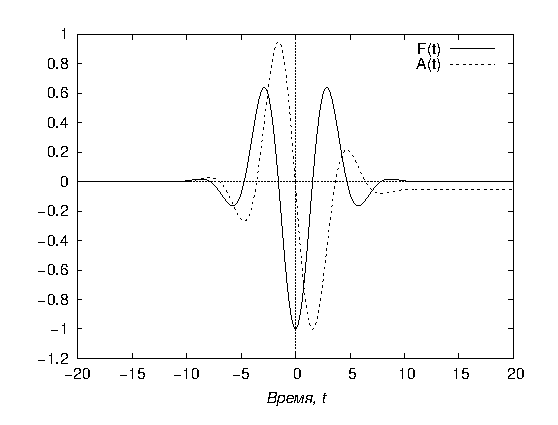
\includegraphics[width=\linewidth]{F_A}}
	\caption{Функции $F(t)$ и $A(t)$}
	\label{ris:f_a}
\end{figure}

\sectionbreak

\section{Описание метода перевала} 

В данной главе дается основное содержание метода перевала для оценки интеграла вида~\ref{eq:input}.
 
Метод перевала применяется для оценки при больших значениях параметра $\lambda$ контурных интегралов вида
\begin{equation}\label{eq:eq6}
I(\lambda) = \int_{C}^{}\phi(t)e^{\lambda f(z)}dz,
\end{equation} 
где $f(z)$ и $\phi(z)$ функции, аналитические вдоль линии интегрирования $С$. Интегралы вида (\ref{eq:eq6}) встречаются также при представлении многих специальных функций, решении дифференциальных уравнений, как обыкновенных, так и с частными производными~\cite{Urmat}.

Рассмотрим частный случай, а именно - действительные интегралы вида

\begin{equation}\label{eq:eq7}
I(\lambda) = \int_{a}^{b}\phi(t)e^{\lambda f(t)}dt.
\end{equation} 

Предположим, что $f(t)$ имеет на отрезке $(a, b)$ один резко выраженный максимум. Чем больше значение параметра $\lambda$, тем резче выражается этот максимум, и поэтому ясно, что при больших $\lambda$ основной вклад в значение интеграла дает окрестность точки максимума. 

В основе этого метода лежит лемма:

\textit{Лемма \label{lemma:lemma1}}: Пусть дан интеграл

$$
I(\lambda) = \int_{0}^{a}\phi(t)e^{-\lambda t^\alpha}dt \:\:\:\:\:\: (0 < a \le \infty, \alpha>0),
$$
где $\phi(t)$ при $|t|<2h$ представляется сходящимся рядом

$$
\phi(t)=t^\beta(c_0+c_1 t+\dots+c_n t^n+\dots), \; \beta>-1,
$$
причем $\int_{0}^{a}|\phi(t)| e^{-\lambda_0 t^\alpha}dt\le M$ для некоторого $\lambda_0$. Тогда имеет место асимптотическое разложение

\begin{equation}\label{eq:eq8}
I(\lambda) \sim \sum_{n=0}^{\infty}\frac{c_n}{\alpha} \Gamma\left(\frac{\beta + n + 1}{\alpha}\right)\lambda^{-\frac{\beta + n + 1}{\alpha}},
\end{equation} 
где $\Gamma$ - гамма-функция Эйлера.

К доказанной лемме сводится оценка интеграла (\ref{eq:eq7}).

\textit{Теорема 1\label{th:th1}}. Пусть интеграл (\ref{eq:eq7}) абсолютно сходится для некоторого $\lambda = \lambda_0$, т. е.
$$
\int_{a}^{b} |\phi(t)|e^{\lambda_0 f(t)}dt \le M,
$$
и $f(t)$ достигает своего наибольшего значения во внутренней точке $t_0$ отрезка $(а, b)$, в окрестности $| t - t_0| < \delta$ которой $f(t)$ представляется рядом
$$
f(t)=f(t_0) + a_2(t-t_0)^2+\dots+a_n(t-t_0)^n+\dots \;\; (a_2<0),
$$
причем существует $h > 0$ такое, что вне этой окрестности $f (t_0) — f(t) > h$. Пусть еще функция $t = \psi(\tau)$ определяется в окрестности точки $\tau = 0$ из уравнения $f(t_0) — f(t) = \tau^2$, причем в этой окрестности
\begin{equation}\label{eq:eq9}
\phi[\psi(\tau)]\psi^\prime(\tau) = \sum_{n=0}^{\infty} c_n\tau^n.
\end{equation}

Тогда интеграл (\ref{eq:eq7}) имеет асимптотическое разложение
$$
I(\lambda)=\int_{a}^{b}\phi(t)e^{\lambda f(t)}dt \sim e^\lambda f(t_0) \sqrt{\frac{\pi}{\lambda}} \sum_{n=0}^{\infty}\frac{c_2n}{\lambda^n}\frac{(2n)!}{4^n n!}.
$$

Эта теорема относится к случаю, когда наибольшее значение $f(t)$ достигается во внутренней точке отрезка $(a, b)$. 

\textit{Теорема 2\label{th:th2}}. Пусть интеграл (\ref{eq:eq7}) абсолютно сходится для некоторого $\lambda = \lambda_0$ (см теорему 1) и $f(t)$ достигает наибольшего значения в точке $t=a$, аналитична в этой точке ($f^\prime(a) \neq 0$), и существует $h>0$ такое, что $f(a)-f(t)>h$ вне некоторой окрестности точки a. пусть еще функция $t=\psi(t)$ определяется в окрестности точки $\tau=0$ из уравнения $f(a) - f(t) = \tau$, причем в этой окрестности имеет место разложение (\ref{eq:eq9}). Тогда

\begin{equation}\label{eq:eq10}
I(\lambda) = \int_{a}^{b}\phi(t)e^{\lambda f(t)}dt \sim \frac{e^{f(a)}}{\lambda}\sum_{n=0}^{\infty}\frac{n! c_n}{\lambda^n}.
\end{equation}

Суть метода перевала состоит в том, что при больших значениях параметра $\lambda$ величина интеграла

$$
I(\lambda) = \int_{C}^{}\phi(t)e^{\lambda f(z)}dz
$$
в основном определяется тем участком пути интегрирования $C$, на котором $|e^{\lambda f(z)}|=e^{\lambda \Re f(z)}$, т. е. $\Re f(z)$ велика по сравнению со значениями на остальной части $С$. При этом интеграл оценивается тем легче, чем меньше этот участок и чем круче падает величина $\Re f(z)$ В соответствии со сказанным, при применении метода перевала стараются деформировать путь интегрирования С в наиболее удобный путь $\widetilde{C}$, пользуясь тем, что по теореме Коши такая деформация не меняет величины интеграла.\cite{Urmat}

Для геометрической иллюстрации метода положим $z = x + iy$, и представим
$$
u = \Re f(z),
$$
как поверхность $S$ в пространстве $(x, y, u)$. Так как функция $u$ гармоническая, то $S$ не может иметь точек максимума и минимума, а точки, в которых $f'(z) = 0$, будут для нее точками перевала (седловыми точками, рисунок \ref{ris:image2}).

\begin{figure}[h]
	\center{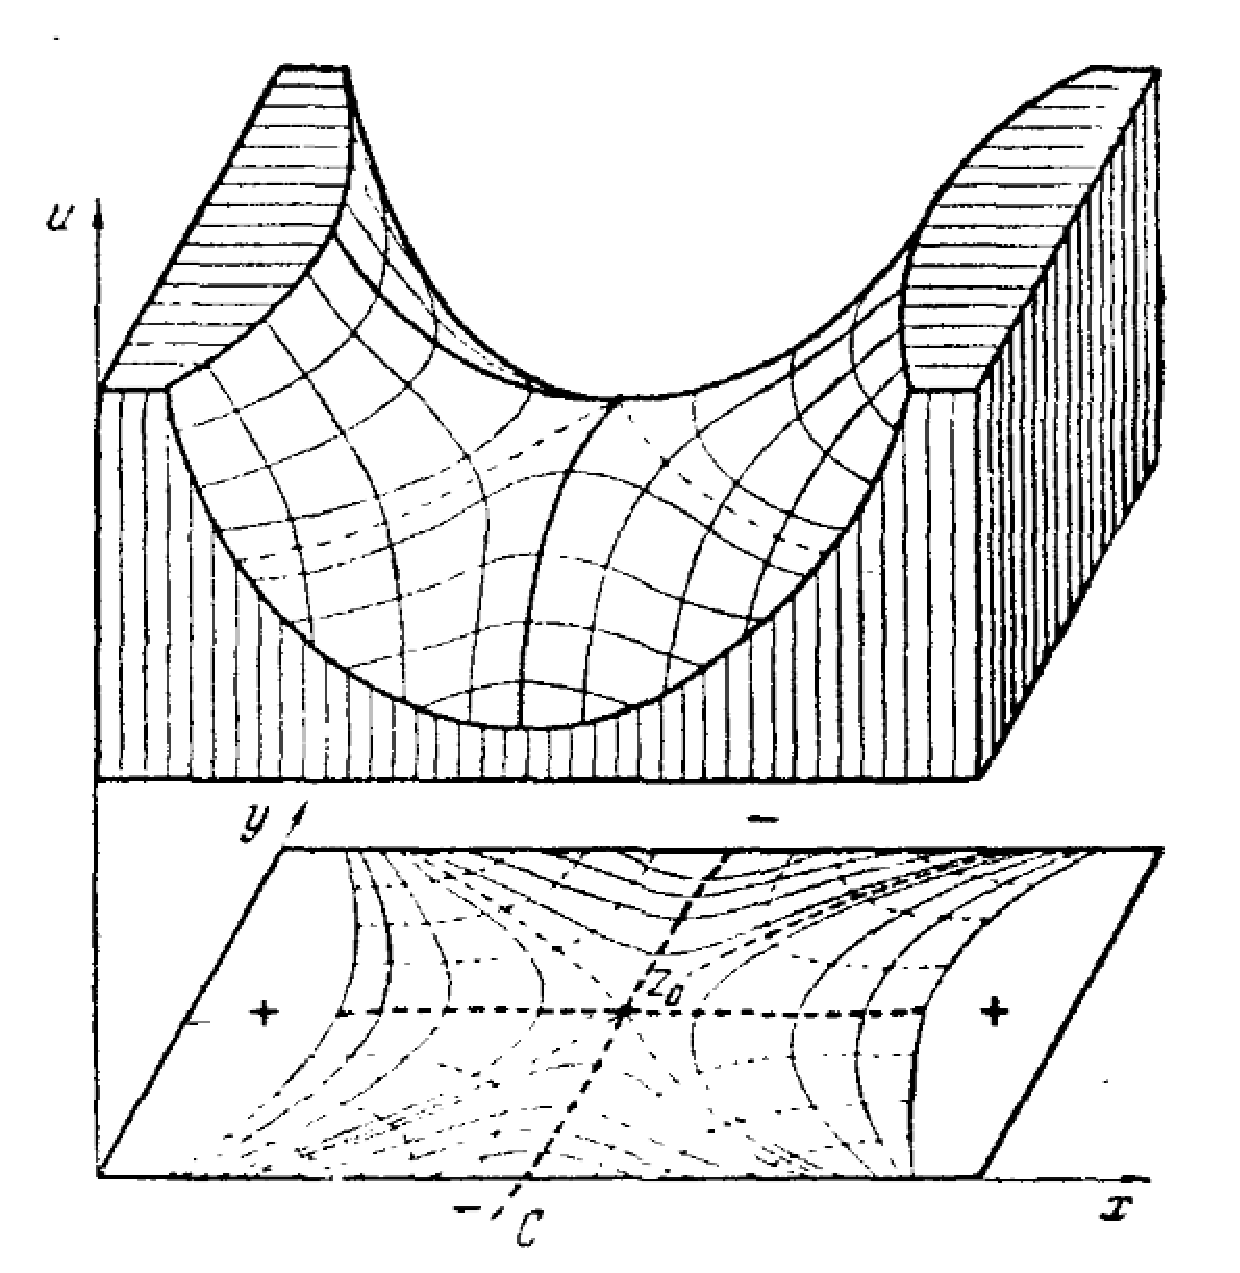
\includegraphics[width=0.6\linewidth]{pic2}}
	\caption{Седловые точки}
	\label{ris:image2}
	\end{figure}

Наиболее удобный для оценки путь интегрирования $\widetilde{C}$, в каждой точке должен проходить в направлении наиболее быстрого изменения $\Re f(z)$, а так как функция f(z) аналитическая, то это направление должно совпадать с линией, на которой $\Im f(z) = \const$. 

Также, новый контур $\widetilde{C}$ должен содержать точку $z_0$, в которой $\Re f(z)$ достигает наибольшего значения на $\widetilde{C}$. Покажем для этого случая, что $f^\prime (z_0) = 0$, то есть точка линии $\Im f(z) = \const$, в которой $\Re f (z)$ достигает наибольшего значения, является точкой перевала.

Так и есть, ведь в точке $z_0$, которая является максимумом для $\Re f (z)$ производная $u=0$ вдоль линии $\widetilde{C}$ должна быть равна 0, т. е. $\frac{\partial}{\partial s}\Re f(z)=0$, а так как $\Im f(z) = \const$ на $\widetilde{C}$, то $\frac{\partial}{\partial s} \Im f(z) \equiv = 0$, а значит и 

$$
f^\prime(z_0) = \frac{\partial}{\partial s} \Re f(z) + i\frac{\partial}{\partial s} \Im f(z) = 0.
$$ 

\textit{Для метода перевала к интегралу (\ref{eq:eq6}) путь интегрирования $С$ следует деформировать в путь $\widetilde{C}$, проходящий через точку перевала $z_0$ и в окрестности этой точки идущий вдоль линии наибольшего ската $\Im f(z) = \const$ (рисунок \ref{ris:image2}).}

Есть одно важное обстоятельство, обеспечивающее эффективность применения метода перевала: так как вдоль линии $\widetilde{C}$ имеем $\arg e^{f(z)} = \Im f(z) = \const$, то оценка интеграла (\ref{eq:eq6}) сводится к оценке интеграла от действительной функции, которая может быть проведена по методу Лапласа для интеграла вида (\ref{eq:eq7}).  \cite{Fedoryuk}

Именно это позволяет нам пользоваться полученными результатами теорем 1 и 2. 

Рассмотрим  случай, когда путь интегрирования $С$ можно деформировать в путь $\widetilde{C}$, проходящий через точку перевала $z_0$, где $f^\prime(z_0) = 0$, $f^{\prime\prime}(z_0)\neq0$, и в окрестности $z_0$ совпадающий с линией наибольшего ската $\Im f(z) = \const$, причем на $\widetilde{C}$ вне этой окрестности $\Re f(z) < \Re f(z_0) - h \;(h> 0)$. Кроме того, предположим, что интеграл (\ref{eq:eq6}) абсолютно сходится для достаточно больших значений $\lambda$.
Тогда образом, оценку интеграла можно провести на основании теоремы 1. Пусть $z = z(t)$ будет уравнение контура $\widetilde{C}$; Тогда,

\begin{equation}\label{eq:eq11}
I(\lambda) = \int_{C}^{}\phi(z) e^{\lambda f(z)}dz=e^{\lambda i \Im f[z(t)]}\int_{a}^{b}\phi[z(t)]e^{\lambda \Re f[z(t)]}z^{\prime} dt.
\end{equation}

и задача сводится к оценки интеграла вида $\ref{eq:eq7}$ действительной области, разложение для которого уже было получено Лапласом, и имеет вид \cite{Wong}:

$$
I(\lambda) = \int_{a}^{b}\phi(t)e^{\lambda f(t)}dt \sim \frac{e^{f(a)}}{\lambda}\sum_{n=0}^{\infty}\frac{n! c_n}{\lambda^n}.
$$

Выпишем первый член этого разложения. Обозначим $\phi[z(t)]z^\prime = \widetilde{\phi}(t)$, $\Re f[z(t)] = \widetilde{f}(t)$ и тогда по формуле (\ref{eq:eq10}) получаем:

\begin{equation}\label{eq:eq12}
\int_{a}^{b} \widetilde{\phi}(t) e^{\lambda \widetilde{f}(t)}dt \sim e^{\lambda \widetilde{f}(t_0)} \sqrt{\frac{\pi}{\lambda}} \widetilde{c_0},
\end{equation}
где $\widetilde{c_0}$ - свободный член в разложении функции $\widetilde{\phi}[\widetilde{\psi}(\tau)]\widetilde{\psi^\prime}(\tau)$.

Имеем: $\widetilde{\phi}(t_0) = \phi(z_0) z^\prime (t_0)$, и исходя из того, что $f[z(t)] = \Re f[z(t)]+ i \Im f[z(t)] = \widetilde{f}(t)+\const$ вдоль $\widetilde{C}$, то

\begin{equation}\nonumber
\widetilde{f}^{\prime\prime} (t_0) = \frac{d^2}{d t^2} f[z(t)]\;|_{t=t_0} = f^{\prime\prime} (z_0) z^{\prime^2} (t_0),
\end{equation}
причем $f^\prime[z(t)] z^{\prime \prime} (t) = 0$ при $t=t_0$. Так как эта величина отрицательна, то представив $z^\prime (t_0) = k e^{i \theta}$, можно записать ее в виде $\widetilde{f}^{\prime\prime}=-|f^{\prime\prime}(z_0)| k^2$. Получаем, что 

\begin{equation}\nonumber
\widetilde{c}_0=\widetilde{\phi}(t_0) \sqrt{-\frac{2}{\widetilde{f}^{\prime\prime}(z_0)}}= \phi (z_0) e^{i \theta} \sqrt{\frac{2}{|f^{\prime\prime}(z_0)|}}.
\end{equation}
Подставим найденное значение в (\ref{eq:eq12}), а затем в (\ref{eq:eq11}), получаем искомую формулу

\begin{equation}\label{eq:eq13}
I(\lambda) \sim e^{\lambda f (z_0)}\sqrt{\frac{2\pi}{|f^{\prime \prime} (z_0)|}} \phi(z_0) e^{i \theta} \frac{1}{\sqrt{\lambda}}.
\end{equation}

Как говорилось ранее, точка $z_0$ - это точка, где $\Re f(z)$ достигает своего максимального значения. В то же время совершенно обычная ситуация - когда на искомом контуре $\widetilde{C}$ имеется несколько точек перевала, в которых значения $\Re f (z)$ находятся вблизи к наибольшему, то следует взять сумму выражений (\ref{eq:eq13}) по всем этим точками. 

Тот случай, когда контур интегрирования заканчивается в точке перевала $z_0$, аналогичным образом приводится к теореме \ref{th:th2}.

Итак, мы получили рабочую формулу, подставляя в которую составляющие наших искомых функций $\phi (z)$ и $f (z)$, мы должны получать приближенные значения интеграла, когда $\lambda \rightarrow \infty$ 

В интеграле $\cM(\epsilon,t)$ (\ref{eq:input}) роль большого параметра $\lambda$ играет величина:

\begin{equation}\label{eq.lambda}
\lambda = \frac{1}{2 \cT} \int_{-\cT/2}^{\cT/2} A^2(\tau) d\tau.
\end{equation}

\sectionbreak
\section{Методы вычисления функции $\cM(\epsilon,t)$}
\subsection{Аналитическое решение}
Получим формулу оценки интеграла (\ref{eq:input}) при помощи метода перевала.

Прежде всего заметим, что наряду с перевальными точками вклад в интеграл может давать значение $t'=t$, при котором следует учитывать ``сингулярность'' в подынтегральной функции $\sim (t-t')^{-3/2}$. Однако, вклад окрестности $t'=t$ может рассматриваться независимо от вклада перевальных точек, ввиду того, что функция $S(t', t)$ при $t'\to t$ мала, и метод перевала становится несправедлив.

Функция $S(t', t)$ при фиксированном $t$ показана на рисунке~\ref{ris:S}.
Из рисунка (\ref{ris:S}) видно, что большое значение функция $S$ может принимать только в случае $|t - t'|\gg 1 $. 

\begin{figure}[h]
	\center{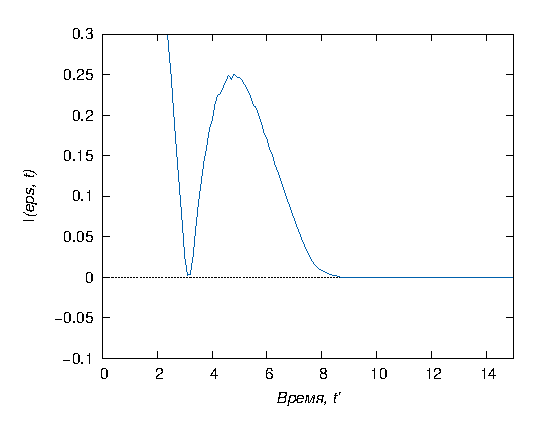
\includegraphics[width=\linewidth]{S}}
	\caption{Значение функции $S(t', t)$ для t=-20, 0 и 20}
	\label{ris:S}
\end{figure}


Рассмотрим случай $t \to t'$ отдельно. В этом случае разложение функции $S$ в ряд Тейлора принимает вид

$$ 
S(t', t) \sim \frac{1}{24} \left( \frac{d}{dt}A(t)\right)^{2}(t' - t)^3 + \frac{1}{24} \frac{d}{dt}A(t) \cdot \frac{d^2}{dt^2}A(t) (t' - t)^4 + \ldots
$$
В первом неисчезающем порядке, учитывая $F(t)=-\dot{A}(t)$:
\begin{equation}\label{eq:S_0}
S(t', t) \sim \frac{F^{2}(t)}{24}(t' - t)^3.
\end{equation}
Подставляя (\ref{eq:S_0}) в интеграл (\ref{eq:input}) для $\cM$ и вводя замену $t - t' = \tau$, получаем 

\begin{eqnarray}
\cM_{\tau = 0} = \frac{1}{\sqrt{2\pi i}} \int_{0}^{\infty} \frac{e^{i \epsilon \tau}}{\tau^{3/2}} \left(e^{-i \frac{А^2(t)}{24} \tau^3} - 1\right) d\tau  = \nonumber \\
= \frac{1}{\sqrt{2\pi i}} \int_{0}^{\infty} e^{i \epsilon \tau} \tau^{3/2} d\tau \cdot \left(-i\frac{F^2(t)}{24}\right) 
\label{int:tau0}
\end{eqnarray}

На рисунке \ref{ris:I_0} отображен график $\cM_{\tau = 0}(\epsilon,t)$. 
Полученная функция, как видно из графика, очень быстро затухает. Поскольку при недостаточном отдалении от нуля ($t \approx 0$) даже для функции $S(t', t)$ малый размер функции не позволяет использовать перевальную оценку, то вкладом $\cM_{\tau = 0}(\epsilon, t)$ вблизи нуля, а также на остальном участке можно пренебречь (на интервале $t = (10, \infty)$: $\cM_{\tau = 0}(\epsilon, t) \approx 0$).  

\begin{figure}[h]
	\center{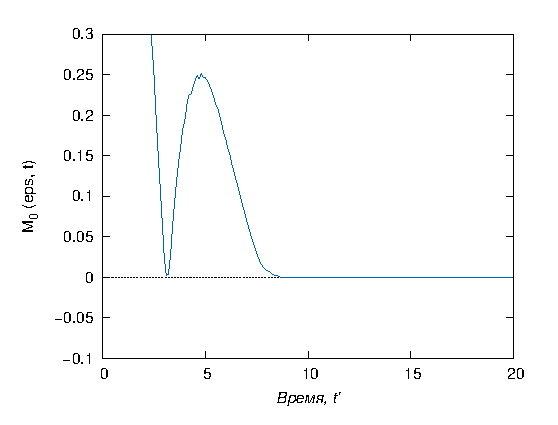
\includegraphics[width=\linewidth]{I_0}}
	\caption{Вклад интеграла $\cM_{\tau = 0}(\epsilon, t)$}
	\label{ris:I_0}
\end{figure}


Для учета перевальных точек рассмотрим интеграл:
$$
\cM \sim \int_{-\infty}^{t} \frac{1}{(t-t')^{3/2}} e^{i[\epsilon (t - t') + S(t, t')]} dt',
$$
где опущено второе слагаемое -1 в (\ref{eq:input}), регуляризующее сингулярность $(t-t')^{-3/2}$. Как следует из оценки $\cM_{\tau = 0}$
это слагаемое не существенно в области применимости метода перевала.

После замены $t - t' = \tau$, получаем 
$$
\cM \sim \int_{0}^{\infty}\frac{1}{{\tau}^{3/2}}e^{i [\epsilon \tau + S(t, t-\tau)]} d\tau.
$$

Если обозначить
$
f(t, \tau) = \epsilon \tau + S(t, t-\tau) 
$ и
$
\phi(\tau) = \frac{1}{{\tau}^{3/2}} 
$, то получим формулу вида:
$$
\cM \sim \int_{0}^{\infty} \phi(\tau) e^{i f(t, \tau)} d\tau,
$$
которая формально совпадает с рассмотренным в главе 2 интегралом (\ref{eq:eq6}).

В результате применения метода перевала, получаем:
\begin{equation}
\label{an.res1}
\cM(\epsilon, t) \simeq \sqrt{\frac{1}{2\pi i }}\sum_{\tau_0}e^{f(t, \tau_0)} \sqrt{-\frac{2}{\partial^2 f(t, \tau)/\partial \tau^2|_{\tau = \tau_0}}} \phi(t_0),
\end{equation}
где $\tau_0$ - корни уравнения $\partial f(t,\tau)/\partial \tau = 0$.

Найдем выражение для $\partial^2 f(t, \tau)/\partial \tau^2$ и решим уравнение на стационарные точки $\tau_0\equiv t-t_0$.

Дифференцируя $
f(t, \tau) = \epsilon \tau + S(t, t-\tau),
$ по $\tau$ получим:

$$
\frac{\partial f(t, \tau)}{\partial \tau} = \epsilon + \frac{\partial S(t, t-\tau)}{\partial\tau},
$$
\begin{equation}\label{eq:points}
\frac{\partial f(t, \tau)}{\partial \tau}=0\;\; \Rightarrow \;\; \frac{\partial S(t, t-\tau)}{\partial\tau} = -\epsilon.
\end{equation}
С введенной заменой $S$ примет вид
$$
S(t, t-\tau) = -\frac{1}{2}\int_{t-\tau}^{t} \alpha(\epsilon, t, t-\tau)^2 d\epsilon
$$
Дифференцируя $S(t, t-\tau)$ по $\tau$, получаем

$$
\frac{\partial S(t, t-\tau)}{\partial\tau} = -\frac{1}{2} \alpha(t-\tau, t, t-\tau)^2.
$$
Произведем обратную замену $t_0 = t-\tau_0$ и с учетом уравнения (\ref{eq:points}), получаем явный вид уравнения на стационарные точки:

\begin{equation}\label{eq:solvepoints}
\alpha ^2 (t_0, t, t_0) = 2 \epsilon.
\end{equation}

Далее получим формулу для $D\equiv\partial^2 f(t, \tau)/\partial\tau^2$:

$$
D = -\frac{1}{2}\left[\alpha(t-\tau, t, t-\tau)^2\right]' = 
-\alpha(t_0, t, t_0) \alpha(t_0, t, t_0)',
$$
и с учетом явного вида $\alpha$~(\ref{eq:alpha}):
\begin{equation*}
D = \alpha(t_0, t, t_0)\left[F(t_0) - \frac{1}{(t - t_0)^2} \int_{t_0}^{t}A(\tau)d\tau +  \frac{A(t_0)}{t-t_0} \right].
\end{equation*}

Подставляя полученные соотношения в формулу~(\ref{an.res1}), получаем:
\begin{equation}\label{eq:out}
\cM(\epsilon, t) \simeq \sum_{t_0}\frac{e^{i\widetilde{S}(t, t_0)} }{\sqrt{D} (t-t_0)^{3/2}},
\end{equation}
где $\widetilde{S} = \epsilon \tau_0 + S(t, t-\tau_0) = \epsilon(t-t_0) + S(t, t_0)$.

Видно, что полученная формула включает в себя множество различных элементов, предполагающих численное интегрирование. Также перед ее вычислением необходимо решать уравнение~(\ref{eq:solvepoints}) на стационарные точки для каждого~$t$.

Прежде всего заметим, что в соответствии с уравнением~(\ref{eq.system}) аргумент $\epsilon$ рассматриваемой функции $\cM(\epsilon,t)$ может принимать любые вещественные значения.
В случае отрицательных $\epsilon$ решения уравнения~(\ref{eq.system}) становятся комплексными, и требуют отдельного детального анализа. 

В данной работе мы ограничимся случаем вещественных точек стационарной фазы ($\Im t_0=0$), и, соответственно, рассмотрим положительные значения $\epsilon>0$.
Из~(\ref{eq:solvepoints}) имеем два уравнения:

$$\alpha(t', t, t') - \sqrt{2\epsilon} = 0,$$
$$\alpha(t', t, t') + \sqrt{2\epsilon} = 0,$$
объединяя все решения которых, получаем искомые седловые точки $t'=t_0$.

Построим график функции $\alpha(t', t, t')$ на отрезке $t' = [-20..20]$ при $t = 0$ (рисунок \ref{ris:alpha-20..0}):
Видно, что корней несколько и они практически симметричны относительно ветвей оси $O y$. Важно, что в суммировании участвуют только решения на промежутке $t' = [-20, t]$. 
На графике показано, что не для каждого $\epsilon$ у нас найдутся решения в области действительных чисел. Максимальное значение $\epsilon$ при данных условиях около 0.6.

\begin{figure}[h]
	\center{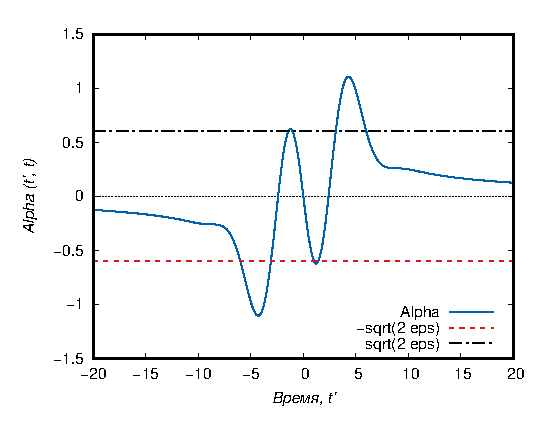
\includegraphics[width=\linewidth]{alpha-200}}
	\caption{Функция $\alpha$ при $t = 0$.}
	\label{ris:alpha-20..0}
\end{figure}



Если корни близки к локальному экстремуму функции $\alpha(t', t, t')$, то возможен случай слияний корней, который является еще одним ограничением использования перевальных оценок.
Чтобы этого избежать, можно получить оценку не для двух точек, а для одной, которая находится между ними на равном удалении: равномерная аппроксимация исходного интеграла~\cite{Fedoryuk}.
В этом случае асимптотическое разложение интеграла $\cM$ примет другой вид в связи с тем, что сделанное ранее предположение о равенстве нулю первой производной фазовой функции в подынтегральном выражении будет не верным. Оценка $\cM$ при равномерной аппроксимации выражается через функцию Эйри~\cite{spec}. Поскольку явный вид ее объемный, приведен он не будет, но получение не вызывает трудностей.

На рисунке \ref{ris:alpha-20..20} представлен график $\alpha(t', t, t')$ на отрезке $t' = [-20..20]$ при $t = 20$. С ростом $t$ 
корней становится меньше, и они дальше друг от друга расположены, чем на рисунке~\ref{ris:alpha-20..0}. Следует заметить, что для каждого значения $\epsilon$ необходимо проверять существование решения уравнения на рассматриваемом временном интервале.
В данной работе для нахождения корней уравнений используется метод Брента~\cite{tarasevych}.


\begin{figure}[h]
	\center{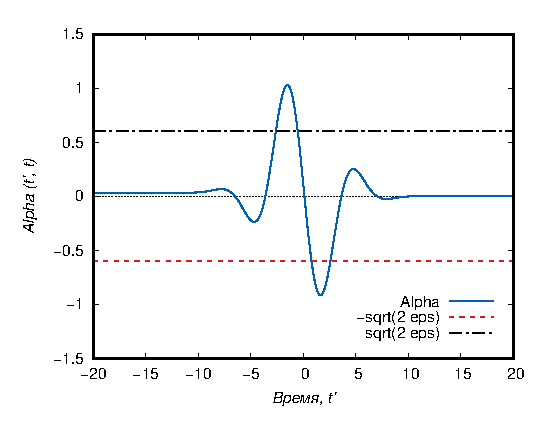
\includegraphics[width=\linewidth]{alpha-2020}}
	\caption{Функция $\alpha$ при $t = 20$.}
	\label{ris:alpha-20..20}
\end{figure}


В общем случае корни седлового уравнения могут быть комплексные. Тогда необходимо решать систему (при фиксированном $t$):

\begin{eqnarray}
\begin{cases}
\Re \ \alpha(x+i y, t, x+i y) = 2\epsilon \nonumber\\
\Im \ \alpha(x+i y, t, x+i y) = 0 \nonumber
\end{cases}
\end{eqnarray}
Здесь $\epsilon$ - любое действительное число. В этом случае потребуется производить интегрирование в области комплексных чисел, что вызывает определенные трудности. Проблема также возникает в поиске множества корней. Основным методом решения уравнений в нескольких измерениях является метод градиентного спуска, то есть должны быть описаны также производные этих функций. Самым трудоемким в таком случае является именно поиск множества корней, так как возможна потеря некоторых из них во время перехода к следующей области поиска.

\sectionbreak

\subsection{Численное решение}

В данной главе обсуждается алгоритм вычисления выражения (\ref{eq:input}) непосредственным интегрированием несобственного интеграла.


Нижняя граница $t_b$ интервалов интегрирования для интегралов от величин, определяемых функциями $F(t)$ или $A(t)$ с ограниченным носителем (см. выражение~(\ref{eq:f}) и рисунок~\ref{F-A}) определяется заданной точностью $\delta$, в соответствии с условием

$$
\exp( -t_b^2/a^2) < \delta.
$$

Например, интеграл (\ref{eq:a}) принимает вид:

$$\label{eq:easy}
A(t) = -\int_{t_b}^{t} F(\tau) d\tau.
$$
Для вычисления этого интеграла воспользуемся гауссовскими квадратурами:
$$
\int_{x_1}^{x_2} f(x) dx = \sum_{j=1}^{N} \omega_j f(x_j),
$$
с весами $\omega_j$ и узлами $x_j$, явный вид которых приведен в~\cite{spec}. 

Для реализации вычисления интегралов, определяющих классическое действие $S(t',t)$ [которое в свою очередь входит в подынтегральную функцию для искомой величины $\cM(\epsilon,t)$~(\ref{eq:input})] необходимо адаптировать гауссовские методы интегрирования под переменные пределы интегрирования и требуемую точность.  Для этих целей воспользуемся библиотекой подпрограмм GSL (GNU Scientific Library)~\cite{gsl:website}. 

GSL - это открытая библиотека, написанная на языке программирования C для численных вычислений в прикладной математике и науке.

\textbf{Особенности GSL}: 
\begin{enumerate}
\item библиотека написана полностью для стандарта C (также применима для C++) и основана на использовании заголовочных файлов;
\item определяет новые типы, и структуры данных, у которых нет аналогов в Фортране или C;
\item использует порядок хранения данных на многомерных массивах, отличающийся от используемого Фортраном. 
Единственный способ, использование его в Фортране, состоит в том, чтобы написать собственные подпрограммы на C для обеспечения необходимого соответствия между типами данных, структурами и соглашениями хранения их для двух языков.
\item Интерфейсный уровень не поставляется с библиотекой. 
\end{enumerate}
Самый главный плюс GSL -- скорость вычислений, а также относительная экономия памяти и очистка неиспользуемой памяти. В ней реализовано огромное количество численных методов:
\begin{enumerate} 
	\item Базовые математические функции.
	\item Комплексные числа.
	\item Специальные функции.
	\item Вектора и матрицы.
	\item Комбинаторика.
	\item Сортировка.
	\item Линейная алгебра.
	\item Быстрое преобразование Фурье.
	\item Численно интегрирование (основанное на пакете QUADPACK).
	\item Поиск корней уравнений и др.
\end{enumerate}

Для нашей задачи важны две функции GSL: 

\textit{gsl\_integration\_qags} \cite{gsl:website2}, позволяющая интегрировать функцию на отрезке с заданной точностью, и 

\textit{gsl\_root\_fsolver}, решающая уравнения методом Брента, не используя информацию о производной функции, задающей решаемое уравнение\cite{gsl:website2}.

Максимальная достигнутая точность вычисления интеграла~(\ref{eq:a}) с использованием средств GSL составила $\sim 10^{-9}$.

Для вычисления величины $S(t', t)$ представим её в следующем  виде:

\begin{equation}\label{eq:s_integrate2}
S(t, t') = \frac{1}{2}\int_{t'}^{t} \left( A(\epsilon) - A_1(t', t) \right)^2 d\epsilon,
\end{equation}
где $A_1(t', t) = (t'-t)^{-1}\int_{t'}^{t}A(\tau) d\tau$. Относительно внешнего интеграла по $\epsilon$ $A_1(t', t)$ остается постоянной, поэтому этот элемент можно посчитать только 1 раз для данных $t'$, $t$. Этим преобразованием мы уменьшаем количество операций. 

Основную численную сложность представляет расчет внешнего интеграла~\ref{eq:input} по переменной $t'$ для $M(\epsilon,t)$. 
Для его вычисления используем алгоритм на базе быстрого преобразования Фурье.

Преобразование Фурье переводит функцию времени (временной сигнал) в спектральное (частотное) распределение:
\begin{equation}
\label{int:Fourier}
\hat{f}(\xi) =\int_{-\infty}^{\infty}f(x)e^{-2\pi ix\xi }\,dx.
\end{equation}

При замене непрерывной функции ее отсчетами, вычисленными в дискретные моменты времени, соответствующее преобразование называется дискретным преобразованием Фурье (ДПФ). Для равномерной сетки размера $N$ ДПФ выражается в виде обрезанного ряда Фурье следующего вида:
\begin{equation}
\label{DFT}
X_{k}=\sum_{n=0}^{N-1} x_{n} e^{-i2\pi kn/N},
\end{equation}
Ширина спектра ДПФ является обратной величиной к длительности временного сигнала. Если исходная последовательность охватывает все ненулевые значения функции, ее ДПФ непрерывно и периодично.

Алгоритм быстрого преобразования Фурье (БПФ) вычисляет ДПФ последовательности $X_k$ или обратное ДПФ. Алгоритм БПФ вычисляет такие преобразования, разлагая матрицу ДПФ на произведение разреженных сомножителей. В результате это приводит к уменьшению сложности вычислений ДПФ до $\mathcal{O}(N\log N)$.

Вычисление интеграла (\ref{eq:input}) или (заменяя $t - t' \to \tau$)
\begin{equation}\label{eq:fourier}
\cM (\epsilon,t) = \frac{1}{\sqrt{2\pi i}}\int_{0}^{\infty}\frac{e^{i\epsilon \tau}}{{\tau}^{3/2}}(e^{i S(t, t-\tau)} - 1) d\tau,
\end{equation}
выполним используя алгоритм БПФ.

Для этого воспользуемся программной библиотекой для дискретных преобразований Фурье FFTW~\cite{fftw:website}.
Библиотека FFTW известна как открытая реализация самых быстрых алгоритмов преобразования Фурье (по регулярным сравнительным тестам). 
Одними из плюсов FFTW является адаптивный подбор алгоритма преобразования и возможность сохранения результатов работы библиотеки при многократном повторении ДПФ для последующего использования алгоритма.

С точки зрения практических вычислений, скорость FFTW является определяющим фактором. Возможность сохранения результатов компиляции программы не столь значительна, ввиду малого времени компиляции и слабой зависимости сложности скомпилированного кода программы от вычислительной сложности алгоритма. Основную сложность вычислений составляет не преобразование Фурье, а исходной получение последовательности, над которой выполняется преобразование.

Сравнивая (\ref{eq:fourier}) с (\ref{int:Fourier}), следует положить
$$ 
f(\tau) = \frac{1}{{\tau}^{3/2}}(e^{i S(t, t-\tau)} - 1),
$$
и
$$
\hat{f}(\xi) = \int_{0}^{\infty} e^{i \tau \xi} f(\tau) d\tau.
$$
Тогда 
$$
\cM(\epsilon,t)=\frac{1}{\sqrt{2\pi i}} \hat{f}(\epsilon).
$$
Учитывая, что FFTW реализует дискретное преобразование, значение $\epsilon$ может не совпасть с одной из частот преобразования, попадая в интервал $w_1<\epsilon<w_2$ Для устранения этой проблемы используется следующая линейная аппроксимация спектра:

\begin{equation}\label{eq:approx}
\sqrt{2\pi i}\cM(\epsilon,t) = \frac{(\epsilon - w_1) [\hat{f}(w_2) - \hat{f}(w_1)]}{w_2 - w_1} + \hat{f}(w_1).
\end{equation}

Отметим также, что использование ДПФ для вычисления интеграла~(\ref{eq:input}) позволяет получить за время одного преобразования полный спетр значений функции $\cM(\epsilon)$.

Для проверки точности интегрирования в зависимости от объема дискретизации подынтегральной функции (или размера сетки, или, фактически, верхней границы интервала интегрирования в~(\ref{eq:fourier})), были произведены расчеты для разных значений $N$ при фиксированном шаге дискретизации переменной $\tau$. На рисунке~(\ref{ris:fftw_compare}) изображены результаты численного интегрирования с использованием FFTW для интервалов интегрирования  разной длинны (100 или 200). 
Как видно из рисунка, отличие результатов для различных верхних границ интегрирования достаточно велико. Численный анализ показал, что оптисальным интервалом интегрирования можно считать $[0, 350]$, при котором получается хорошее соотношение между точностью расчетов и затратами.
Кроме того, из рисунка~(\ref{ris:fftw_compare}) видно наличие осцилляций у искомого интеграла, фазы которых зависят от размера интегрируемой области. Причиной тому является особенность ДПФ, а именно его периодичность. Численная ошибка, приводящая к осцилляциям результата, связана с величиной функции $f(\tau)$ на верхней границе интегрирования (в идеальном случае $f(\tau)$ должна обращаться в нуль: $f(0)=f(\infty)=0$).

\begin{figure}[h]
	\center{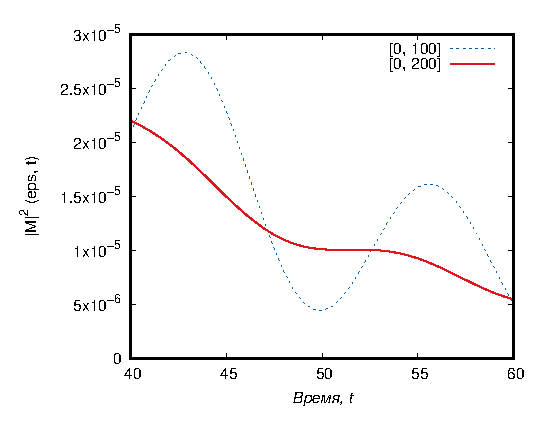
\includegraphics[width=\linewidth]{fftw_compare}}
	\caption{Сравнение результатов интегрирования алгоритмом БПФ для разных отрезков интегрирования}
	\label{ris:fftw_compare}
\end{figure}

Для фиксированного значения параметра $\epsilon$ вместо использования преобразования Фурье, можно воспользоваться другими методами интегрирования. Для сравнения результатов используем интегрирование по методу прямоугольников (т.е. построим прямую интегральную сумму, являющуюся частным случаем ДПФ для нулевой частоты)~\cite{nrc}. Сравнение результата такого интегрирования с результатом, полученным через FFTW показано на 
рисунке~\ref{ris:fftw_compare_no_fftw2}. Отличие представленных на рисунке результатов обусловлено неточностью линейной аппроксимации~(\ref{eq:approx}). Его можно улучшить, используя, например, сплайны второго порядка.

\begin{figure}[h]
	\center{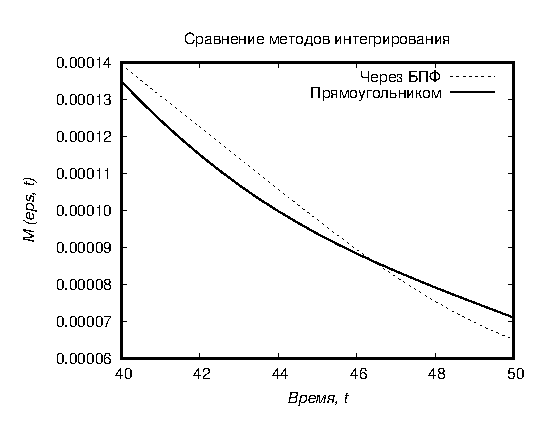
\includegraphics[width=\linewidth]{fftw_compare_nofftw2}}
	\caption{Сравнение результатов для разных методов интегрирования}
	\label{ris:fftw_compare_no_fftw2}
\end{figure}


\sectionbreak
\section{Анализ результатов}

Проведем сравнение аналитического результата~(\ref{eq:out}) для $\cM(\epsilon,t)$ с результатом численного интегрирования исходного интеграла в~(\ref{eq:input}). Для этого произведем вычисления матричного элемента $\cM(\epsilon,t)$ на отрезке $t = [0, 70]$. 
Для больших значений $t$ становятся существенными численные ошибки, ввиду малости значения $\cM(\epsilon,t)$: $\cM(t>70)\sim 10^{-7}$.
При определении параметров поля $F(t)$ в~(\ref{eq:f}), будем полагать ширину огибающей фиксированной ($a^2=20$) и менять амплитуду $F_0$ и несущую частоту $\omega$. 

На рисунке~\ref{ris:roots1} изображены решения седлового уравнения~(\ref{eq:solvepoints}) для следующих параметров:
$\epsilon = 0.4$, $F_0 = 2$, $\omega = 0.8$.
Из графика видно, что для $t>5$ количество различных корней уравнения ровно 4, и с ростом $t$ новых корней не возникает, а значит рассматривать отрезок такой длинны на появление новых корней не имеет смысла.

\begin{figure}[h]
	\center{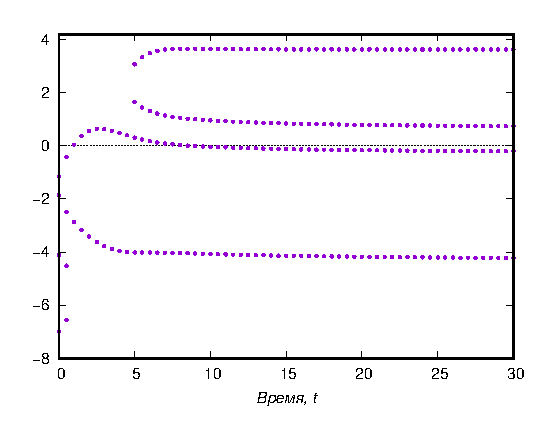
\includegraphics[width=\linewidth]{roots1}}
	\caption{Седловые точки для $\epsilon = 0.4$, $\omega = 0.8$, $F_0=2$.}
	\label{ris:roots1}
\end{figure}

Для выявления общей закономерности появления новых решений уравнения~(\ref{eq:solvepoints}) с ростом $t$ построим график для других значений $\epsilon$ (рисунок \ref{ris:roots2}).
Видно, что для $\epsilon = 0.3$ корней больше, чем для больших значений $\epsilon$: максимум 6, и последний появляется при $t \approx 11$.
При дальнейшем росте $t$ количество решений не возрастает.
Увеличение числа корней с уменьшением $\epsilon$ подтверждается зависимостью $\alpha(t',t,t')$ от $t'$ на рисунке~\ref{ris:alpha-20..20}.

\begin{figure}[h]
	\center{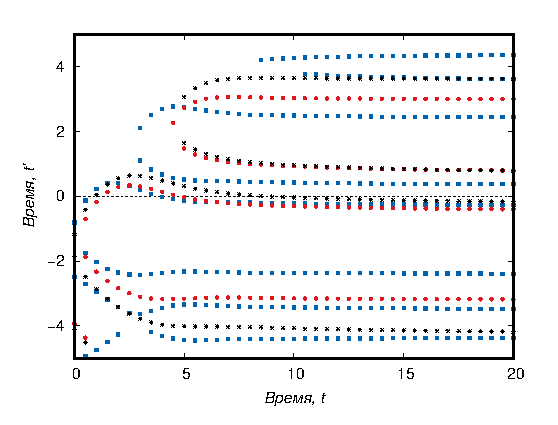
\includegraphics[width=\linewidth]{roots2}}
	\caption{Седловые точки для  $\epsilon = 0.3$ (квадраты), 0.35 (круги) и 0.4 (звездочки). Параметры функции $F(t)$ те же, что на рисунке~\ref{ris:roots1}. }
	\label{ris:roots2}
\end{figure}

Сравнение аналитического и численного результатов для параметров $\epsilon = 0.4$, $F_0 = 2$, $\omega = 0.8$ показано на рисунке \ref{ris:full1}. 
Из рисунка видно, что при малых $t$ в аналитическом решении проявляются пики, отсутствующие в численном решении. Сравнение с рисунком~\ref{ris:roots1} показывает, что положение этих пиков совпадает со значениями $t$, при которых возникают новые решения седлового уравнения. Причин возникновения пиков может быть две: первая связана с тем, что новые решения появляются при $t=t'$, что соответствует сингулярности в подынтегральной функции $\sim(t-t')^{-3/2}$; вторая~-- при появлении решений парами в точке появления они сливаются, в результате чего производная $D$ в выражении~(\ref{eq:out}) для сливающихся седловых точек обращается в нуль, и метод перевала становится не применим. 

\begin{figure}[h]
	\begin{center}
%		\begin{minipage}[h]{0.45\linewidth}
			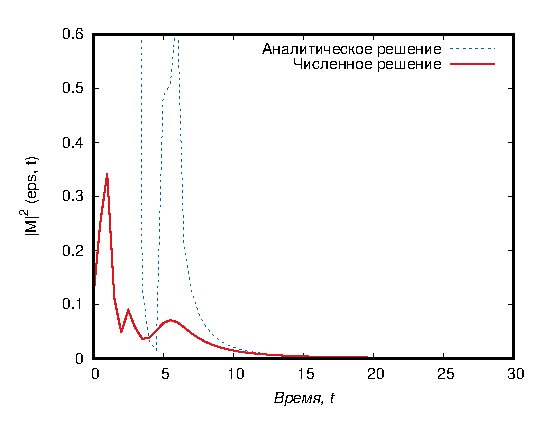
\includegraphics[width=1\linewidth]{full1}
			\caption{Сравнение численного \textit{(сплошная линия)} и аналитического \textit{(пунктирная линия)} результатов на временном отрезке $t\in[0, 30]$ для параметров как на рисунке~\ref{ris:roots1}} %% подпись к рисунку
			\label{ris:full1} %% метка рисунка для ссылки на него
%		\end{minipage}
%		\hfill 
%		\begin{minipage}[h]{0.45\linewidth}
%			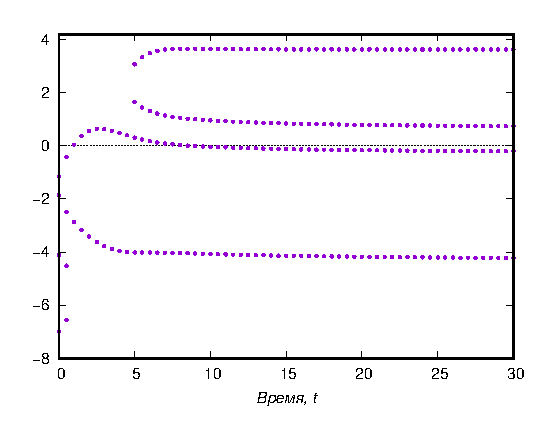
\includegraphics[width=1\linewidth]{rootsend1}
%			\caption{Корни для аналитического решения }
%			\label{ris:rootsend1}
%		\end{minipage}
	\end{center}
\end{figure}

При удалении $t$ от значения перевальной точки $t'=t_0$ аналитическое решение показывает хорошее согласие с численным расчетом. Областью удовлетворительного согласия можно считать $|t-t_0|>2\pi/\omega$, то есть при временном удалении на период поля от перевальной точки $t_0$ поведение матричного элемента $\cM(\epsilon,t)$ хорошо описывается аналитической перевальной оценкой. Согласие аналитического и численного решений при больших значениях $t$ показано на рисунке~\ref{ris:end1}.  Заметим, что расхождение результатов на рисунке~\ref{ris:end1} отчасти связано с неточностью численного решения.

\begin{figure}[h]
	\center{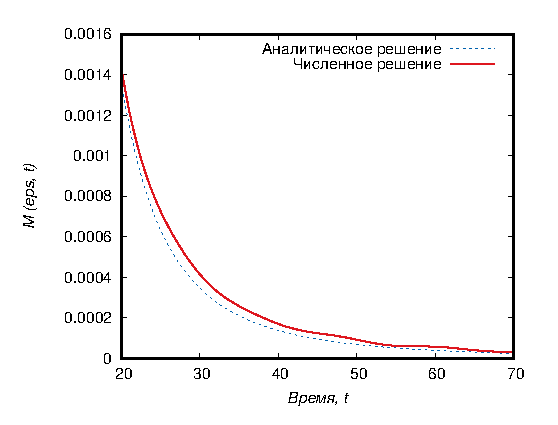
\includegraphics[width=\linewidth]{end1}}
	\caption{То же, что на рисунке~\ref{ris:full1} для $t\in[20, 70]$}
	\label{ris:end1}
\end{figure}

Аналогичное согласие результатов наблюдается и для следующих параметров задачи: $\epsilon = 0.35, F_0 = 2.2, \omega = 0.8$ (см. рисунки \ref{ris:full2} и \ref{ris:end2}).

\begin{figure}[h]
	\begin{center}
%		\begin{minipage}[h]{0.45\linewidth}
			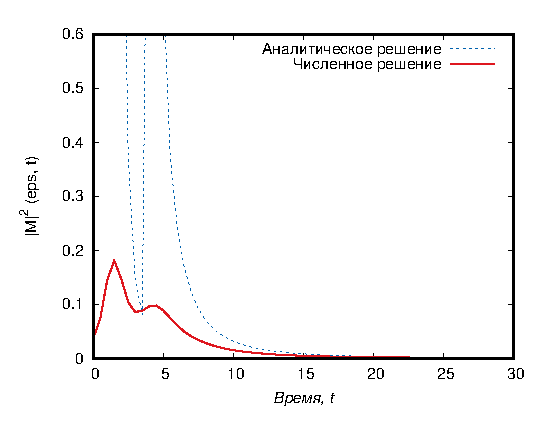
\includegraphics[width=1\linewidth]{full2}
			\caption{Сравнение численного \textit{(сплошная линия)} и аналитического \textit{(пунктирная линия)} результатов на временном отрезке $t\in[0, 30]$ для параметров $\epsilon = 0.35, F_0 = 2.2, \omega = 0.8$} %% подпись к рисунку
			\label{ris:full2} %% метка рисунка для ссылки на него
%		\end{minipage}
%		\hfill 
%		\begin{minipage}[h]{0.45\linewidth}
%			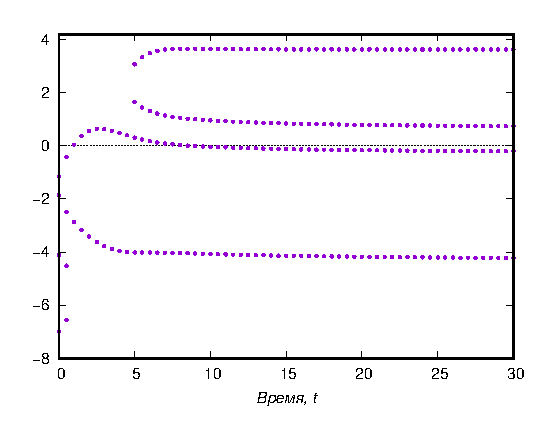
\includegraphics[width=1\linewidth]{rootsend1}
%			\caption{Корни для аналитического решения }
%			\label{ris:rootsend2}
%		\end{minipage}
	\end{center}
\end{figure}

\begin{figure}[h]
	\center{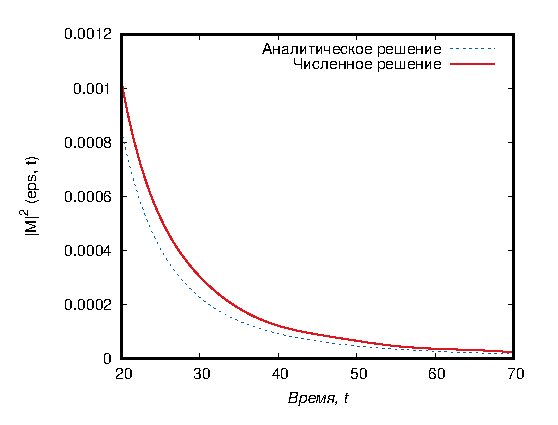
\includegraphics[width=\linewidth]{end2}}
	\caption{То же, что на рисунке~\ref{ris:full2} для $t\in[20, 70]$}
	\label{ris:end2}
\end{figure}

Изменим $F_0$ и получим графики для других параметров задачи: $\epsilon = 0.35, F_0 = 1,6, \omega = 1$ (см. рисунки \ref{ris:full3} и \ref{ris:end3}). Как видно из сравнения рисунков \ref{ris:end1} и \ref{ris:end3}, с уменьшением $F_0$ согласие аналитического и численного результатов становится хуже, поскольку величина $\lambda\propto F_0^2/\omega^2$ [см. (\ref{eq.lambda})] для этих условий перестает быть большим параметром, как требуют условия метода перевала (см. главу 2). 

\begin{figure}[h]
	\begin{center}
		%		\begin{minipage}[h]{0.45\linewidth}
		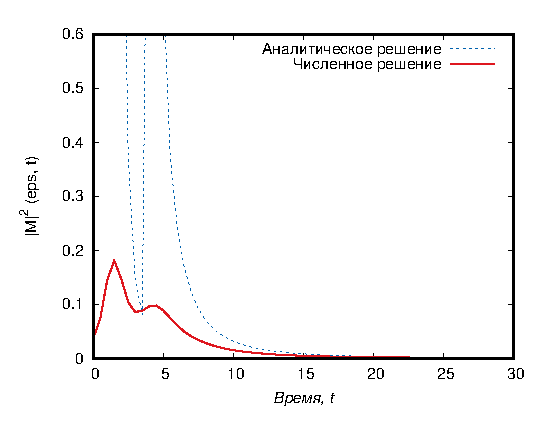
\includegraphics[width=1\linewidth]{full3}
		\caption{Сравнение численного \textit{(сплошная линия)} и аналитического \textit{(пунктирная линия)} результатов на временном отрезке $t\in[0, 30]$ для параметров $\epsilon = 0.35, F_0 = 1,6, \omega = 1$} %% подпись к рисунку
		\label{ris:full3} %% метка рисунка для ссылки на него
		%		\end{minipage}
		%		\hfill 
		%		\begin{minipage}[h]{0.45\linewidth}
		%			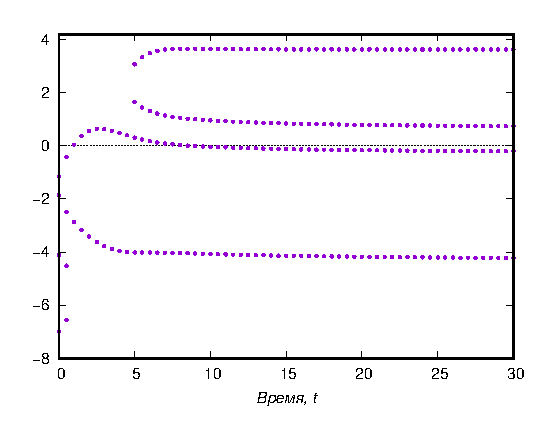
\includegraphics[width=1\linewidth]{rootsend1}
		%			\caption{Корни для аналитического решения }
		%			\label{ris:rootsend2}
		%		\end{minipage}
	\end{center}
\end{figure}

\begin{figure}[h]
	\center{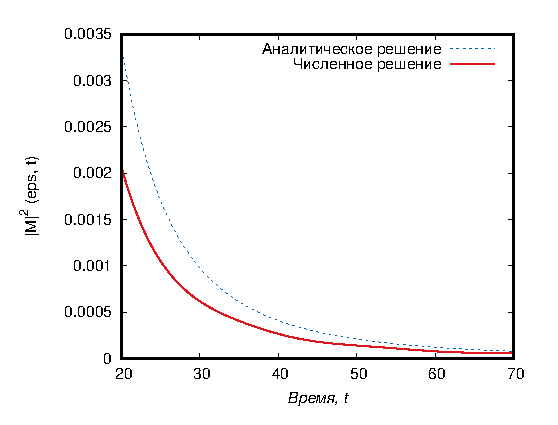
\includegraphics[width=\linewidth]{end3}}
	\caption{То же, что на рисунке~\ref{ris:full3} для $t\in[20, 70]$}
	\label{ris:end3}
\end{figure}

В заключение отметим, что с точки зрения времени вычислений при использовании аналитического результата и прямого численного интегрирования аналитическая формула дает выигрыш во времени на порядок величины. Этот результат можно улучшить, используя для поиска корней седлового уравнения более быстрые алгоритмы, чем метод Брента.

\sectionbreak
\section*{\centering{Заключение}}
\addcontentsline{toc}{section}{Заключение}

В ходе выполнения данной бакалаврской работы рассматривалась задача моделирования взаимодействия атома с полем лазерного импульса. Были получены следующие результаты:
\begin{enumerate}
\item
Получена аналитическая перевальная оценка~(\ref{eq:out}) для матричного элемента $\cM(\epsilon,t)$, определяющего поведение волновой функции атомного электрона,  на малых расстояниях от атома. Результат представляет собой сумму по перевальным точкам слагаемых, каждое из которых выражается через классические физические величины.
\item 
Для получения численной оценки полученной аналитической формулы реализован алгоритм решения нелинейного трансцендентного уравнения, в общем случае имеющего произвольное число корней.
\item 
Разработан и реализован программный модуль на языке C++ для численного нахождения $\cM(\epsilon,t)$ в соответствии с исходным выражением~(\ref{eq:input}). Метод численного решения включает в себя использование гауссовских квадратур и алгоритма быстрого преобразования Фурье.
\item
Проведено численное сравнение результатов аналитического и численного решений. Выявлены границы применимости метода перевала для оценки $\cM(\epsilon,t)$. Обнаружено хорошее согласие аналитического результата с численным для времен $t$, удаленных от значения перевальной точки $t_0$ на величину $|t-t_0|\gtrsim T$, где $T$~-- период колебаний лазерного поля.
\end{enumerate}

Обнаруженное отличие аналитического результата от численного в окрестности $t\approx t_0$ может быть устранено уточнением аналитической оценки, путем более аккуратного учета вклада в оцениваемый интеграл граничной точки $t=t'$ [см. (\ref{eq:input}) и (\ref{int:tau0})], а также использования равномерного приближения для исходного интеграла, учитывающего вклад сливающихся перевальных точек.


\newpage
\addcontentsline{toc}{section}{Список используемой литературы}
\bibliographystyle{ugost2003}
\bibliography{biblio}
% имя библиографической базы (bib-файла) 

\newpage
\addcontentsline{toc}{section}{Приложение А Листинг программы}
\section*{Приложение А\\Листинг программы}\label{attachA}

В данном приложении приведен текст программы, реализующей алгоритмы, описанные в данной работе.

\lstinputlisting[language=C]{main.c}

\end{document} 